\subsection{Benchmarks}\label{ss:benchmarks}

In order to evaluate different execution modes (bit-level arithmetic and bridging), we use six data-oblivious benchmarks, some of which were adapted from the TERMinator Suite \cite{terminator}. \iffalse , while others were included based on their use in FHE applications. \fi These benchmarks are developed to be data-oblivious and manipulate sets of encrypted variables adjusted to $\{4, 8, 16\}$-bit size.
The algorithms are: (FIB) Fibonacci, an additive-intensive algorithm, (LOG) Logistic Regression, where the data must be capped before inference, (MAX) Maximum, commonly used as non-linear function in ML applications, (MUX) Multiplexer, a simple operation similar to the ternary operator that replaces branch conditions on encrypted data, (PKS) Private Keyword Search, which searches privately for an item in a list or database, and (SOR) Sort, a sorting algorithm with low multiplicative depth, designed for FHE.

% The algorithms are: (FIB) Fibonacci, an additive-intensive algorithm that we use as example in this manuscript, (LOG) Logistic Regression, where the data must be capped before inference, (MAX) Maximum, commonly used as non-linear function in machine learning applications, (MUX) Multiplexer, a simple operation similar to the ternary operator that replaces branch conditions on encrypted data, (PKS) Private Keyword Search, which searches privately for an item in a list or database, and (SOR) Sort, a sorting algorithm with low multiplicative depth specifically designed for FHE.
% The source code of all benchmarks with and without bridging is available in the Appendix.

\begin{figure}[t]
    % \vspace{-0.2cm}
	\centering
    \frame{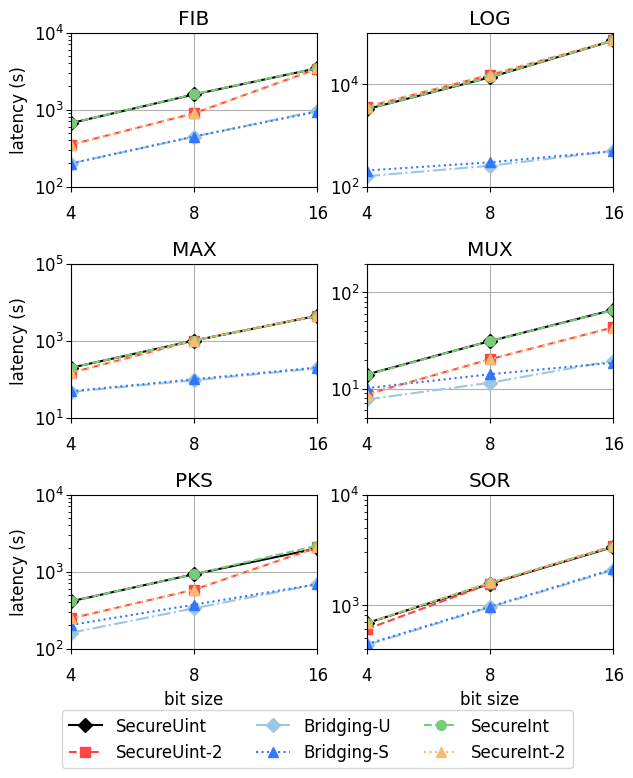
\includegraphics[width=\linewidth]{img/cases_latency.png}}
	\caption{Latency time for six benchmarks\iffalse using \secuint, \secint, unsigned and signed bridging, \texttt{Bridging-U} and \texttt{Bridging-S}, respectively,\fi with $t=2^{16}+1$. \iffalse In addition, we evaluate the benchmarks using \secuint\ and \secint\ with $t=2$ (postfix \texttt{-2}). \fi}
	\label{fig:benchmarks}
	\vspace{-0.4cm} 
\end{figure}

\innersection{Effect of plaintext modulus} Although $t=2$ does not enable batching in BFV, and therefore, it would not be used in practice, we compare it against the smallest plaintext modulus that enables batching ($t=2^{16}+1$) for $n=2^{15}$. The plaintext modulus does not affect the latency time to execute a homomorphic operation, but some homomorphic gates simplify in modulo 2 (e.g. XOR), as we discuss in Section \ref{ss:modcom}. Thus, a Boolean circuit used in bit-level arithmetic should have lower latency for $t=2$ if it contains XOR or XNOR gates. In Fig. \ref{fig:benchmarks}, we can see that in fact some applications are faster in modulo 2 (\texttt{SecureUint-2} and \texttt{SecureInt-2} for unsigned and signed bit-level arithmetic with $t=2$). MUX is the simplest benchmark, containing in bit-level arithmetic one equality, two \secbool-\secuint\ multiplications (or \secbool-\secint\ for signed numbers), one negation, and one addition. A \secbool-\secuint\ multiplication is entirely composed of XOR gates, and around half of the gates in the equality are XOR or XNOR. These operations are mainly responsible for the speed-up. 

% We have a similar situation for FIB and PKS, however here there are relatively fewer \secbool-\secuint\ multiplications and more additions, diminishing the effect of operating in modulo 2. The other benchmarks are much more complex applications and we noticed no difference in latency time between $t=2$ and $t=2^{16}+1$.

\innersection{Bit-level arithmetic vs bridging} Fig. \ref{fig:benchmarks} presents the latency time comparison between bit-level arithmetic and bridging. Regarding unsigned numbers (\secuint\ vs \texttt{Bridging-U}), results show that bridging outperforms bit-level arithmetic for all benchmarks and bit sizes. For some applications, like SOR, the performance improvement is limited (around 60\% speed-up). This happens because this algorithm requires many non-native operations (comparisons) in most stages. Only in the last part of the algorithm bridging can be employed, since using bridging before would require the inefficient conversion from \secmod\ to \secuint\ in order to execute the latter comparisons. Conversely, the logistic regression benefits a lot from using bridging with a speed-up of more than two orders of magnitude. This is possible because the non-native operations required by the filtering function are executed first. Therefore, at the filtering stage it is already possible to employ bridging and perform the remaining computation using the faster modular arithmetic.

\innersection{Signed numbers} Also in Fig. \ref{fig:benchmarks} we compare how bridging behaves with signed numbers. \iffalse In general, the extra conversion time required for signed numbers has little effect in the latency since the application uses significantly more multiplications compared to all the conversions. \fi We can see some degradation in PKS (4 bits) and MUX (4 and 8 bits). In PKS, there is conversion from \secint\ to \secmod\ in every iteration of the loop. The slowest operation in the loop is the comparison. This comparison operation is faster for smaller circuits (4 bits); therefore, the proportional latency of the two ciphertext multiplications required for the \secint\ to \secmod\ conversion is higher. For larger circuits, the comparison becomes more costly, thus, amortizing the conversion cost.

% Regarding MUX, it is a very simple function. It consists only of a comparison followed by a selection of one of two items. The explanation is similar to PKS, but the signed conversion has a higher impact in the latency time because there are two conversions instead of one in this algorithm.

\begin{figure}[t]
    % \vspace{-0.2cm}
	\centering
    \frame{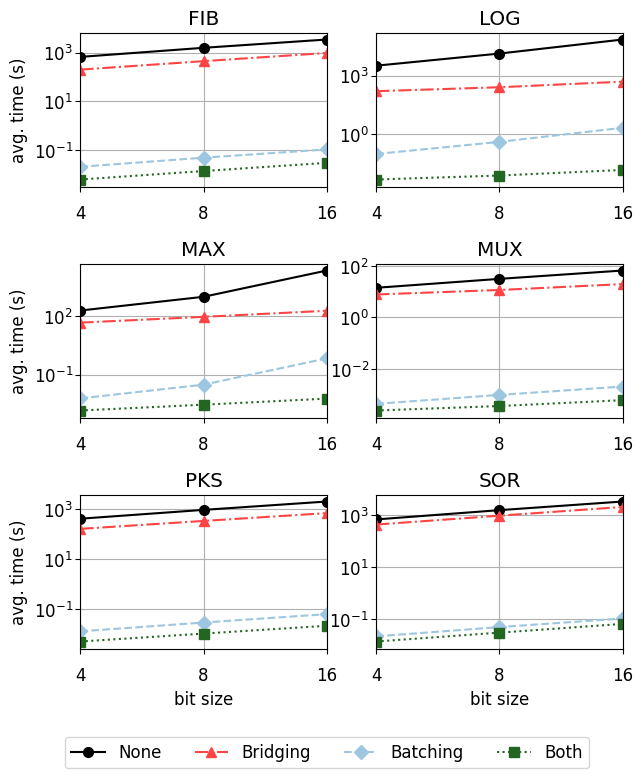
\includegraphics[width=\linewidth]{img/batching.png}}
	\caption{Average execution time for six benchmarks. \iffalse using and four cases: \texttt{None}: without bridging and batching, \texttt{Bridging}: with bridging only, \texttt{Batching}: with batching only, and \texttt{Both}: with both bridging and batching.\fi}
	\label{fig:batching}
	\vspace{-0.4cm} 
\end{figure}



\innersection{Bridging can be used with batching} Batching is a powerful technique used in FHE to pack many plaintexts into a ciphertext. The number of plaintexts that can be packed into a ciphertext is equal to the polynomial degree ($n = 2^{15}$ in our case). Although carefully crafted algorithms using batching and rotations can reduce program latency, the main benefit of batching is increased throughput, since it is possible to process $n$ plaintexts at once. Bridging on the other hand always reduces latency, and consequently improves throughput.
Bridging is a technique independent of batching and both can be used in tandem.
In Fig. \ref{fig:batching} we present the average execution time ($\text{latency} / \text{\# plaintexts packed}$) for six benchmarks and four cases: no batching and no bridging (\texttt{None}), bridging-only (\texttt{Bridging}), batching-only (\texttt{Batching}), and batching and bridging together (\texttt{Both}).
As expected, the throughput improvement provided by batching is impressive. However, for this technique to be used at its fullest, it is necessary to fill all ciphertext slots with plaintexts, which is the case with embarrassingly parallel workload. If the load is less than $n$, the performance will degrade.
Bridging does not suffer from this problem since it focuses on reducing the latency.
Nevertheless, bridging can be used in combination with batching. In this case, the speed-up of both techniques is added, leading to an even faster runtime (acceleration by more than 6 orders of magnitude (LOG)).

\innersection{Insights}
Bridging demonstrates substantial performance improvement for algorithms that allow mixing \secuint{} and \secmod{}, while in the worst case, bridging is equivalent to bit-level arithmetic. \iffalse This would happen if all outputs of a program come out from non-native operations. \fi
The comparison heavy SOR benefits less from bridging since these operations occur throughout the program and near the output, which precludes using the \secmod{} type in an earlier stage. On the contrary the benchmarks containing non-native operations near the beginning exhibit more significant performance improvements (MAX, FIB, PKS).
\iffalse At first glance, the MAX algorithm looks similar to SOR. However, some subtle differences in the \texttt{selection} function allow us to use bridging much earlier in the program; in fact, near the beginning of the application, leading to a much more noticeable performance improvement. 
FIB, and PKS have comparisons in all iterations, but since these comparisons are at the beginning of each iteration, bridging provides substantial performance improvements. \fi
Bridging benefits are maximized when non-native operations (e.g. comparisons) are at the beginning of the computation and the remaining of the computation can be done in modular arithmetic. The non-native operation would require the whole computation to work on bit-level arithmetic, but with bridging it becomes much faster since only the non-native operations are performed with \secuint, while the remaining run using \secmod. This is demonstrated by our logistic regression benchmark, which provides more than two orders of magnitude (precisely 143 times) of performance improvement.

% Finally, it is possible to combine bridging with batching for further performance improvement since both techniques are orthogonal to each other. It should be noted that this performance improvement is tightly connected to the parallelization capabilities of the workload. Nevertheless, results show that some benchmarks, when \emph{both} batching and bridging are combined, can be accelerated by more than 6 orders of magnitude (LOG).

\vspace{-0.1cm}